% %%% Time-stamp: <2023-11-16 14:56:49 vladimir>
% %%% Copyright (C) 2019-2023 Vladimir G. Ivanović
% %%% Author: Vladimir G. Ivanović <vladimir@acm.org>
% %%% ORCID: https://orcid.org/0000-0002-7802-7970

\chapter{Discussion}%
\label{ch:discussion}%
\noindent\bigskip%

This chapter addresses this dissertation's research question:
\medskip%
\begin{quote}\OnehalfSpacing
  Has Rocketship structured itself to earn a return for its founders and investors, focusing especially on its real estate transactions?
\end{quote}
The chapter looks more closely at the research question and summarizes the key findings of the research. It then discusses what kind of evidence would confirm or disconfirm the research question. It looks at three well-known approaches to making arguments for or against a proposal or policy and uses those approaches to make the case that Rocketship has in fact organized itself to make money and that real estate is the vehicle it uses. The two final sections discuss what policy issues are raised during the examination of the data and the evidence, what further research is warranted. Lastly, this dissertation makes a brief conclusion.

\section{The Research Question}%
\label{sec:research-question}\indent%

The research question really is asking three questions:
\begin{enumerate}
  \item Has Rocketship structured itself to make money?
  \item If so, is real estate the vehicle that Rocketship uses to make money?
  \item Is this Rocketship's intent?
\end{enumerate}

2015section{Key Findings}%
\label{sec:summary-key-findings}\indent%

This dissertation's epigraph is \textit{Cui bono?}. Who does benefit?

After a careful examination of Rocketship's finances, a key finding is that no evidence of illegal activity was uncovered in Rocketship's \textit{publicly available} financial documents. This is fortunate, because California is notorious for charter school fraud. Nine years ago, \textcite{CPD2015} found \$81M in fraud, and in 2019, a single online charter school was discovered to have defrauded the State of California of \$400M. Another report 

The report, \citetitle{CPD2015} estimated in 2015 that ``\ldots{} [t]he vast majority of this fraud perpetuated by charter officials will go undetected because California lacks the oversight necessary to identify the fraud.'' \parencite[2]{CPD2015}. With tens billions of dollars of funding for charter schools in California alone coupled with lax oversight, the temptation must be great. 

There are, however, some questionable expenditures, namely \$2M spent on travel in 2022.

So, who benefits from Rocketship's growth every year in net assets?

\section{Arguments Which Answer the Research Question}%
\label{sec:appr-answ-rese-quest}\indent%

\subsection{Rappaport's Rules}%
\label{sec:rappaports-rules}\indent%

Anatol Rapoport, a [mathematical] game theorist, proposed four rules that seek to increase understanding and avoid defensive responses. \citefirstlastauthor{Dennett2013} reformulated them in his book \citetitle{Dennett2013} \parencite{Dennett2013}:
\begin{enumerate}[topsep=0.3\baselineskip,itemsep=0.25\baselineskip]
  \item You should attempt to re-express your target’s position so clearly, vividly, and fairly that your target says, “Thanks, I wish I’d thought of putting it that way.”
  \item You should list any points of agreement (especially if they are not matters of general or widespread agreement).
  \item You should mention anything you have learned from your target.
  \item Only then are you permitted to say so much as a word of rebuttal or criticism.
\end{enumerate}
\medskip

So, here is the Rocketship Rappaport argument:
\begin{enumerate}[topsep=0.3\baselineskip,itemsep=0.25\baselineskip]
  \item Public schools, in areas of poverty, for whatever reason(s), fail at educating their children well, and they educate children of color especially poorly. We (Rocketship) aim to change this by a combination of focus, targeted intervention, and technology. We are focused on doing whatever it takes to raise the educational attainment of our students, and we focus day in and day out on this one goal. Our pedagogy has two major aspects: We monitor and target with specialize intervention students who are not doing as well as we would like, and we use technology (computer-aided instruction) to tailor instruction to a specific child's needs at exactly the time they need intervention.
  
  We believe that, by controlling our facilities, we can remove a serious distraction that comes with sharing facilities with a public school district. Not only are we not beholden to the whims of the public school district, but we do no have to spend time preparing year after year a Proposition 39 facilities request. We are never embroiled in petty disputes about interactions between public school students and our students because they simply never arise. Our results speak for themselves. All of our schools do better than their surrounding district and do better than the California average.
  \item I agree that some public school districts have failed in their primary duty to educate children, but I attribute that to chronic underfunding and to local and state governments tolerating conditions (crime,drug use,unemployment) that would never be tolerated in suburbia. But, staying the course is not an option because doing the same thing over and over and expecting different results is not likely to be successful, now or ever.
  I also agree that providing separate facilities for children rather than forcing them to share is more likely to be successful than otherwise. Being able to control the school environment brings stability the classroom.
  \item Starting and operating a charter school is not for the faint of heart. Funding for both operation and for facilities is hard to come by, and must be procured before a single student arrives on campus. Facilities need to be constructed or modified well before classes begin. Children need to be enrolled, and parents need to be persuaded to help out. Juggling priorities, contingencies, and expectations is a full-time task, and it shows when the topics of board committee (executive, business, achievement, development) meetings are looked at.
    \item However, even given the truthfulness of the items 1–3 above, there are some areas where criticism, some of it quite severe, is warranted.
    \begin{itemize}[topsep=0.125\baselineskip,itemsep=0.25\baselineskip]
      \item Despite the acknowledged need for independent facilities, Rocketship spends an inordinate amount of time on topics that are not academic in focus. One can see this in the topic areas of its board committees, where only one of four has to do with academic achievement.
      \item Rocketship short-changes current students in order to create future students by allocating 20\% of revenue to facilities. Although this is legal, I suspect that the California Legislature did not expect one charter school to be begetting another, just as the Legislature didn't anticipate the damage that for-profit charter school chains or virtual charter schools would do.
      The percentage of revenue that Rocketship spends on administration (i.e. management), is unusually high at 14\% in 2022 \parencite[38]{RSEA2022}. General administrative expenses in public school districts are in the 5\% to 10\% range. So, right off the top, 35\% of revenue is siphoned off and does not go directly to educating children.
      \item Teachers at Rocketship schools in Santa Clara county have much less experience and are paid substantially less than, say, teachers in the San José Unified School District. If we believe that teachers are a key factor in delivering a quality education, then what kind of teachers Rocketship hires and how much it pays them are important determinants of the quality of the teaching staff and hence how well Rocketship educates its children.
      \item Rocketship has seriously exaggerated how well its students do compared to public school students. The size of the discrepancy, 4× to 5× larger than what was reported in the literature, seems to indicate a certain amount of desperation to convince people that Rocketship is both committed to ``eliminating the achievement gap in our lifetime'' and successful at it.\\
      According to the latest \citetitle{SCCOE2014}, comparing the percentage of Rocketship students who ``met/exceeded standards'' on the Smarter Balanced Summative Assessments (SBAC) test in English Language Arts (ELA) during the 2021-22 school year, only a single Rocketship school (out of eight Santa Clara County authorized schools) did better than public school students in Santa Clara County. In Mathematics, the number of schools who did better was actually less than one; it was zero.\\
      Moving on to comparing how Rocketship schools did against state public schools, only one school exceeded the state average in ELA—by a single percentage point—and five exceeded the state average in Mathematics. Granted, these results are not as bad as ACE Empower that managed only 19\% met or exceeded standards in ELA and 11\% in Mathematics, but for a chain of schools whose goal is to close the achievement gap, Rocketship's scores are not encouraging \parencite{SCCOE2014}.\\
      Also discouraging is the trend in the last five years. In five schools, the percent met/exceeded has fallen in ELA and all but one have fallen in Mathematics. However, a deeper dive into the scores is needed to determine if this because parents with children who were not doing as well as hoped for enrolled and thus brought the average scores down, or whether this is truly a reflection on the effectiveness of Rocketship's pedagogy. More honesty and transparency and less of the cult-like chanting at the start of a school day would be welcome.
      \item Rocketship's policy of owning its facilities has led to over \$185M\footnote{This figure is for all Rocketship schools, i.e. those in  California, Tennessee, Wisconsin, Washington, D.C. and Texas.} in debt, which comes to roughly \$32K per child. At 3\% per annum, that is another \$5.4M that is not going toward educating children.
    \end{itemize}
\end{enumerate}

\subsection{A Toulmin Argument}%
\label{sec:toulmin-arguments}\indent%

Stephen Toulmin was a British philosopher interested in moral reasoning. He developed a method for making practical arguments where ethics and morality played a role. His method has six components, of which the first three are those most commonly seen.
\begin{enumerate}[topsep=0.3\baselineskip,itemsep=0.25\baselineskip]
  \item Claims are statements or conclusions which must be justified.
  \item Grounds are the evidence (facts, data) that provide the basis for making the claim.
  \item Warrants are the connection between the claim and the evidence which backs up the claim.
  \item Backings buttress warrants.
  \item Rebuttals are counter-arguments, made in advance, to potential objections.
  \item Qualifiers express the degree of certainty about the claim.
\end{enumerate}

\prettyref{fig:toulmin-arg} below diagrams the relationship between the parts of a Toulmin argument where rebuttals have been substituted for reservations.

\begin{figure}[ht]
  \caption{The Toulmin Argument Schema}%
  \label{fig:toulmin-arg}%
  \copyrightbox[b]{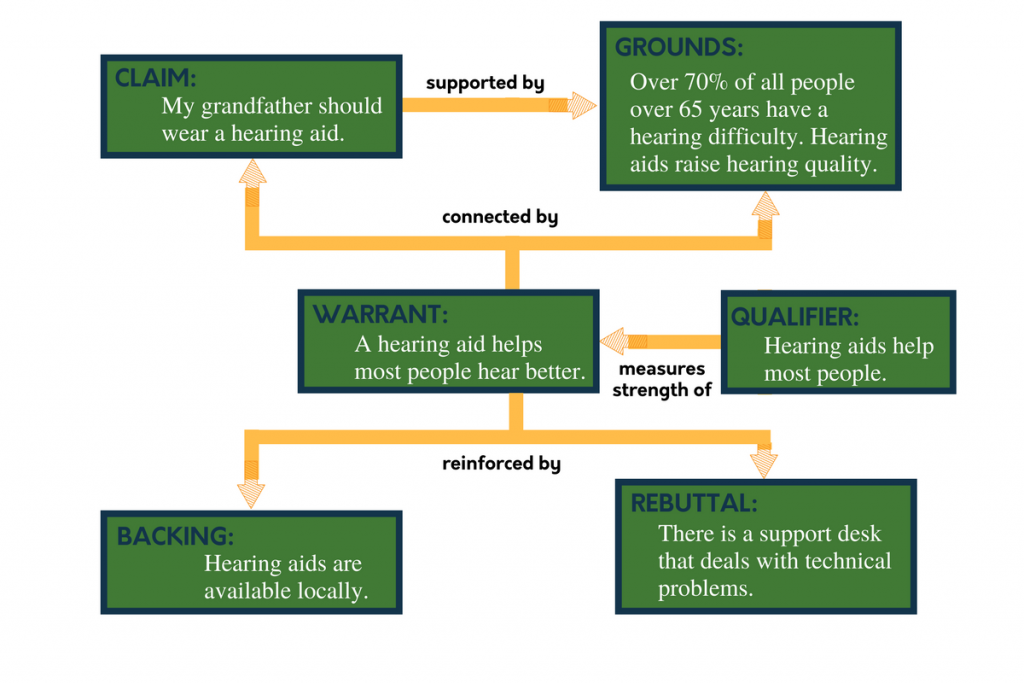
\includegraphics[scale=0.5]{The Toulmin Argument Schema}}{“Toulmin Argument,” Kalyca Schultz, Virginia Western Community College, CC-BY-SA in “Toulmin Argument Model” by Liza Long, Amy Minervini, and Joel Gladd is licensed under CC BY-NC-SA 4.0}
\end{figure}

\paragraph{Claim}
Rocketship is structured to return an as yet unrealized profit to founders and investors, and real estate is the mechanism they are using to turn a profit.
\paragraph{Grounds}
Rocketship's primary focus is not on academic success, but on acquiring real estate. Right from the beginning, Rocketship separated the financing, acquisition, and operation of their facilities from the running of a school; they borrowed heavily and made extensive use of government programs to fund their real estate projects.

Simply judging by the number of board committees devoted to non-academic topics, Rocketship leadership has spent most of their time on real estate issues.

Rocketship has not availed itself (except in one instance) of alternative ways of acquiring facilities. They have not used Proposition 39 to obtain classrooms and fields from a school's home district. They have not tried to convert commercial office space into classrooms. They have not modified existing buildings to serve as schools or classrooms.

Neither the Articles of Incorporation for Rocketship Education nor for Launchpad Development Company contain the language that is present in Summit Public Schools's [Restated] Articles of Incorporation:
\begin{quotation}\noindent%
Article III: The property of this Corporation is \textit{irrevocably} dedicated to charitable purposes and no part of the \textit{net income} or \textit{assets} thereof or to the benefit of private persons except that the Corporation shall be authorized and empowered to pay reasonable compensation for services rendered and to make payments and distributions in furtherance of the purposes set forth in Article II of these Articles of Incorporation. [emphasis added]\sourceatright{\parencite[2]{SummitPublicSchools2017}}
\end{quotation}
The Articles of Incorporation for both Rocketship and Launchpad are possibly equivalent to the first paragraph of Article III of Summit's quoted above, but they are not as explicit or definitive, and they are spread out over several articles and paragraphs.\footnote{Summit makes an exception to the prohibition of private gain for services rendered, which is entirely reasonable. Interestingly, Launchpad's Articles of Incorporation do not, so technically the \$300K paid to Launchpad's CFO \parencite[7]{zotero-16512} in 2019–2020, for example, violates their Articles of Incorporation.}

\paragraph{Warrant}
The best indicators of a firm's real goals are how it spends its time and on what it spends its money, not on what it says.

\section{Answering the Research Question}%
\label{sec:answ-rese-quest}\indent%

As indicated above, this dissertation's research question is actually three sub-questions:
\begin{enumerate}
  \item Has Rocketship structured itself to make money?
  \item If so, is real estate the vehicle that Rocketship uses to make money?
  \item Is this Rocketship's intent?
\end{enumerate}

The arguments given above indicate that the answers are: yes, yes, and yes.

Two questions remain: How and Why? It is not known how the owners and investors of Rocketship going to convert the assets of Rocketship and Launchpad into transferable wealth? Perhaps they do not intend to. Then that begs the question of why. Why is Rocketship accumulating assets. By law and IRS Code they are not allowed to transfer money to a for profit entity. And, probably, they are not allowed to give money to individuals. The only option which makes sense, given the investments of Reed Hastings, Andre Agassi, and the Walton Family Foundation and what has been discovered by this dissertation's investigation is that Rocketship wants to become a self-sufficient charter school incubator for the entire United States.

\section{Public Policy Issues}%
\label{sec:publ-policy-chang}\indent%

\subsection{Fraud}
\label{sec:fraud}

\subsection{Real Estate Conversion}
\label{sec:real-estate-conv}

\begin{quotation}
  Due to a loophole in state law, some private groups have used this public money to buy private property. While charter schools constructed with general obligation bonds cannot be sold or used for anything other than the authorized school, schools constructed with tax-exempt conduit bonds become the private property of the charter operator. Even if the charter is revoked, neither the state nor a local school district can take control of this property. Additionally, schools constructed with private funding subsidized by New Market Tax Credits or acquired with private funds but whose mortgage payments are reimbursed through the Charter Facilities Grant Program (known as “SB740”) are typically owned without restriction. In the event that such schools close down, their owners may be free to turn the buildings into condominiums or retail space, or sell them at a profit. In such cases, neither the school district nor any other public body is entitled to recoup the public dollars that have gone toward creating the facility. \sourceatright{\parencite{IPTP2018}}
\end{quotation}
\begin{itemize}[topsep=0.125\baselineskip,itemsep=0.25\baselineskip]
  \item As far back as 2002, the California State Auditor said, 
  \begin{quote}
    Finding \#3: Chartering entities lacked policies and procedures for fiscal monitoring and have not adequately monitored their charter schools. \sourceatright{\parencite{CAStateAuditor2002}}
  \end{quote}
\end{itemize}

\section{Areas for Future Research}%
\label{sec:issu-future-rese}\indent%

\section{Conclusion}%
\label{sec:conclusion}\indent%


%%% Local Variables:
%%% mode: latex
%%% TeX-master: "Rocketship_Education-An_Exploratory_Public_Policy_Case_Study"
%%% End: